\documentclass{alex_hü}

\name{Alexander Helbok}
\course{PS Physik}
\hwnumber{9}


\begin{document}
\renewcommand{\labelenumi}{\alph{enumi})}


\begin{mybox}{ Wasserstoffatom: Aufenthaltswahrscheinlichkeiten}
	\centering \(  \)
	\tcblower
	\begin{enumerate}
		\item \(  \)
		\begin{minipage}{\textwidth}
			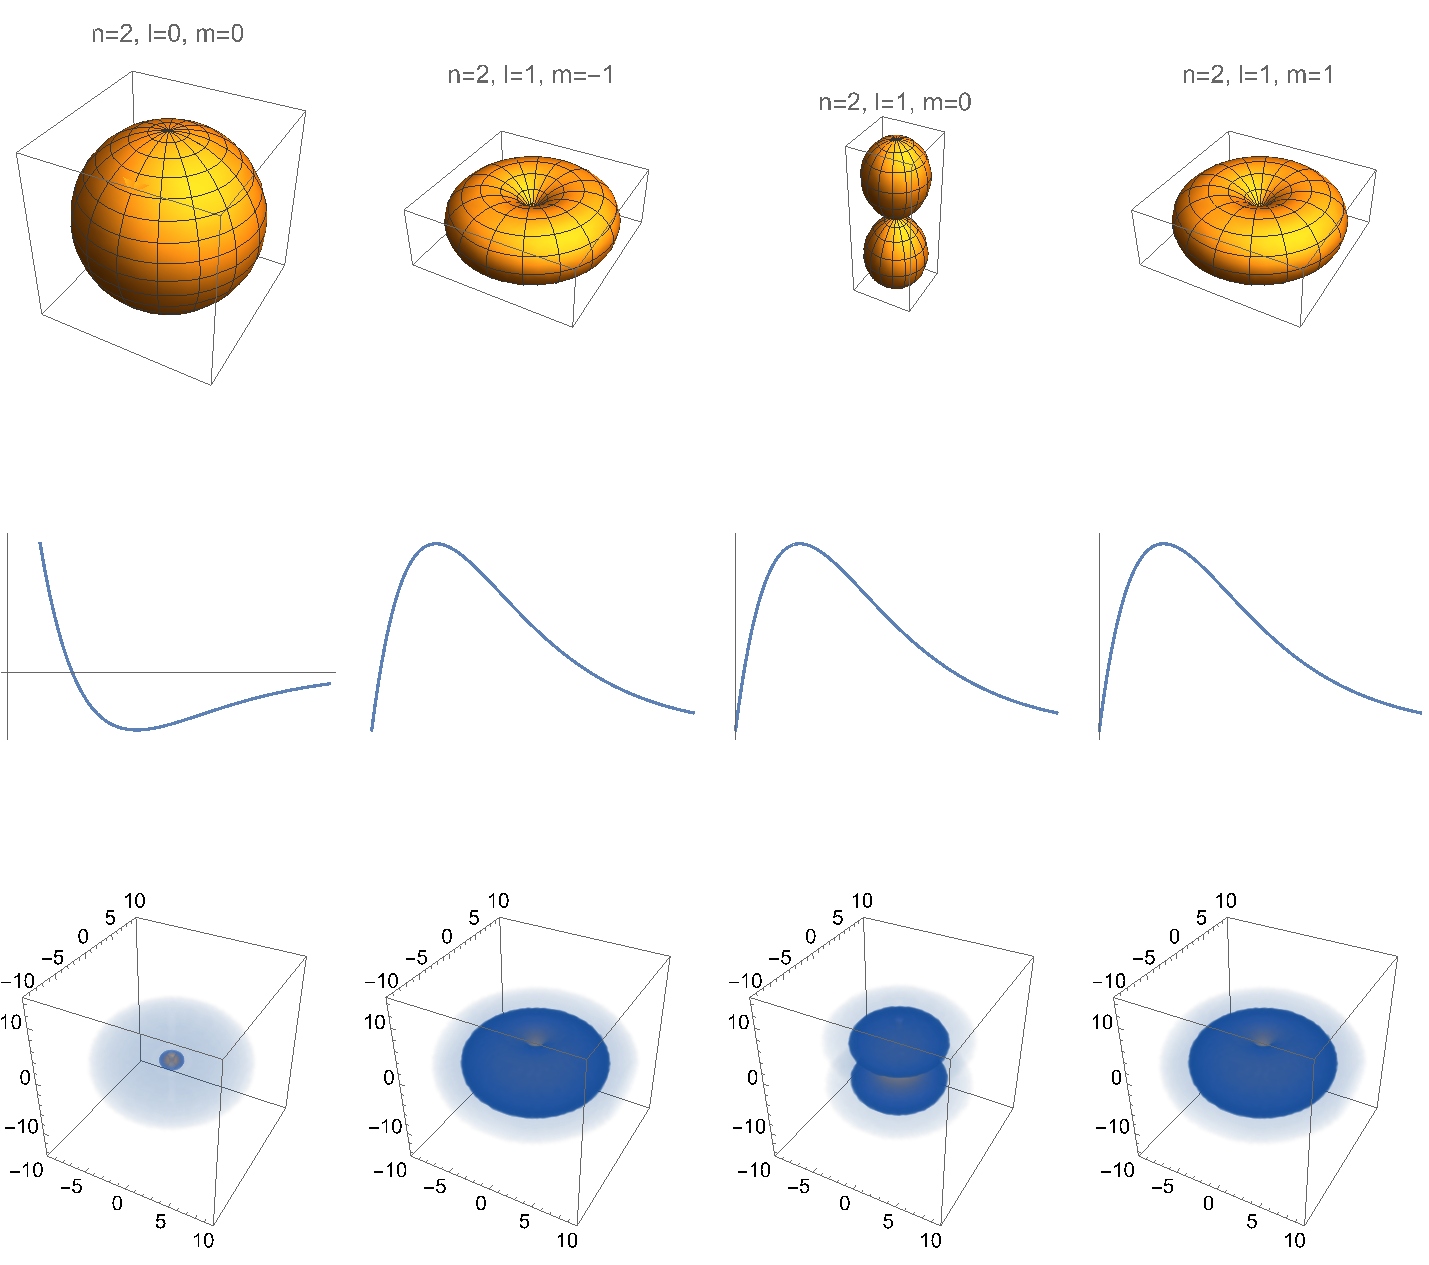
\includegraphics[scale=0.6]{Orbitals}
		\end{minipage}
		
		On top you can see the spherical and radial probability of an electron in a hydrogen Atom for different Quantum numbers. Below is a density plot of the square modulus of the whole wave function (as product of the upper 2 plots). If you sum all 4 states up you can kind of recognize a radial symmetry, as the \( l=0, m=0 \) state is already symmetric and the other three apparently add up to a sphere. 
	\tcbline
		\item \(  \)
		\begin{flalign*}
			\langle \hat{r} \rangle &= \uint[V]{r\abs{\psi_{2,1,1}}^2}{V} = \uint[0,2\pi]{\uint[0,\pi]{\uint[0,\infty]{\frac{1}{24a_0^5}\expo[-][r/a]r^2 \frac{3}{8\pi}\sin(\theta)^2r r^2\sin(\theta)}{r}}{\theta}}{\phi} = &&\\
			&= \frac{1}{32a_0^5} \uint[0,\infty]{r^5\expo[-][r/a_0]}{r} \uint[0,\pi]{\sin(\theta)^3}{\theta} = \frac{1}{32a_0^5}\ 120a_0^6\ \frac{4}{3} = \dl{5a_0} &&\\[1em]
%			
			\langle \hat{r}^2 \rangle &= \uint[V]{r^2\abs{\psi_{2,1,1}}^2}{V} = \frac{1}{32a_0^5} \uint[0,\infty]{r^6\expo[-][r/a_0]}{r} \uint[0,\pi]{\sin(\theta)^3}{\theta} = \dl{30a_0^2} &&\\[1em]
%			
			\langle \Delta\hat{r}^2 \rangle &= \langle \hat{r}^2 \rangle - \langle \hat{r} \rangle^2 = 30a_0^2 - 25a_0^2 = \dl{5a_0^2} &&
		\end{flalign*}
	\tcbline
		\item \( d = 1.75 \unit{fm} \)
		\begin{flalign*}
			P &= \uint[V]{\abs{\psi_{2,0,0}}^2}{V} = \uint[0,2\pi]{\uint[0,\pi]{\uint[0,d]{\frac{1}{4a_0^3}\expo[-][r/a] \left(1-\frac{r}{a_0} + \frac{r^2}{4a_0^2}\right) \frac{1}{4\pi} r^2\sin(\theta)}{r}}{\theta}}{\phi} = &&\\
			&= \frac{1}{2a_0^3} \uint[0,d]{\expo[-][r/a] \left(1-\frac{r}{a_0} + \frac{r^2}{4a_0^2}\right) r^2}{r} = \dl{6.11 \times 10^{-15}} &&
		\end{flalign*}
	\end{enumerate}
\end{mybox}

\begin{mybox}{Drehimpulsquantenzahlen}
	\centering \(  \)
	\tcblower
	\begin{enumerate}
		\item \( \hat{L}_z = -\iu\hbar\pdv{}{\phi};\quad \psi_{n,l,m} = a_m R_{n,l} \cos(\theta)\expo[\iu m\phi]P_l^m \)
		\begin{flalign*}
			\langle \hat{L}_z \rangle &= \uint[V]{\psi^* \hat{L}_z \psi}{V} = -\iu\hbar \uint[V]{\psi^* \pdv{\psi}{\phi}}{V} = \hbar m \uint[V]{\psi^* \psi}{V} = \dl{\hbar m} &&
		\end{flalign*}
	\tcbline
		\item \( \hat{\mathbf{L}}^2Y_l^m(\theta, \phi) = l(l+1)\hbar^2 Y_l^m (\theta, \phi) \)
		\begin{flalign*}
			\langle \hat{\mathbf{L}}^2 \rangle &= \uint[V]{\psi^* \hat{\mathbf{L}}^2 \psi}{V} = \uint[V]{\psi^* R_{n,l} \hat{\mathbf{L}}^2 Y_l^m}{V} = l(l+1)\hbar^2 \uint[V]{\psi^* \psi}{V} = \dl{l(l+1)\hbar^2} &&
		\end{flalign*}
	\tcbline
		\item \(  \)
		\begin{flalign*}
			\left[\hat{\mathbf{L}}^2, \hat{L}_z \right]\psi_{n,l,m} &= \hat{\mathbf{L}}^2 (\hat{L}_z \psi_{n,l,m}) - \hat{L}_z (\hat{\mathbf{L}}^2 \psi_{n,l,m}) = &&\\
			&= \hat{\mathbf{L}}^2 \hbar m\psi_{n,l,m} - \hat{L}_z l(l+1)\hbar^2 \psi_{n,l,m} = &&\\
			&= 
		\end{flalign*}
	\end{enumerate}
\end{mybox}

\begin{mybox}{Zeeman–Effekt}
	\centering \(  \)
	\tcblower
	\begin{enumerate}
		\item \(  \)
%		\begin{flalign*}
		%			
%		\end{flalign*}
	\tcbline
		\item \(  \)
%		\begin{flalign*}
	%		
%		\end{flalign*}
	\tcbline
		\item \(  \)
%		\begin{flalign*}
		%			
%		\end{flalign*}
	\tcbline
		\item \(  \)
%		\begin{flalign*}
	%			
%		\end{flalign*}
	\end{enumerate}
\end{mybox}

\end{document}